% \begin{frame}{Heterogeneous Environment}
%   \begin{table}
%     \centering
%     \begin{tabular}{c c c c}
%       \toprule
%       Device & CPU Speed & Memory & Price \\
%       \midrule
%       Intel NUC & 1.3 GHz & 16 GB & \texttildelow\$300 \\
%       Typical Phones & 2 GHz & 2 GB & \texttildelow\$300 \\
%       Discarded Phones & 1 GHz & 512 MB & \texttildelow\$22 \\
%       BeagleBone Black & 1 GHz & 512 MB & \$55 \\
%       Raspberry Pi & 900 MHz & 512 MB & \$35 \\
%       Arduino Uno & 16 MHz & 512 MB & \texttildelow\$22 \\
%       mbed NXP LPC1768 & 96 MHz & 32 KB & \$10 \\
%       \bottomrule
%     \end{tabular}
%   \end{table}
% \end{frame}

\begin{frame}{Fog/Cloudlet/Swarmbox \& New Infrastructure}
  \begin{columns}
    \column{0.5\textwidth}
    \begin{figure}
      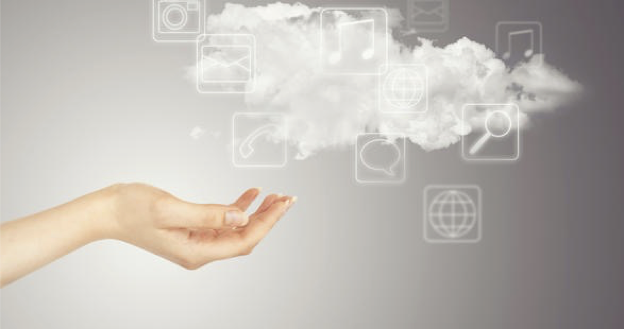
\includegraphics[width=0.8\textwidth]{figures/fog.png}
      \captionsetup{labelformat=empty}
      \caption{Cisco Fog Computing}
    \end{figure}
    \pause
    \column{0.5\textwidth}
    \begin{figure}
      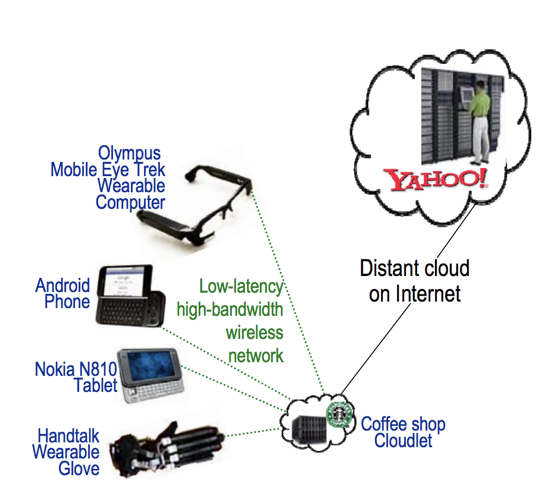
\includegraphics[width=0.8\textwidth]{figures/cloudlet.png}
      \captionsetup{labelformat=empty}
      \caption{CMU Cloudlet}
    \end{figure}
  \end{columns}
  \pause
  \begin{figure}
    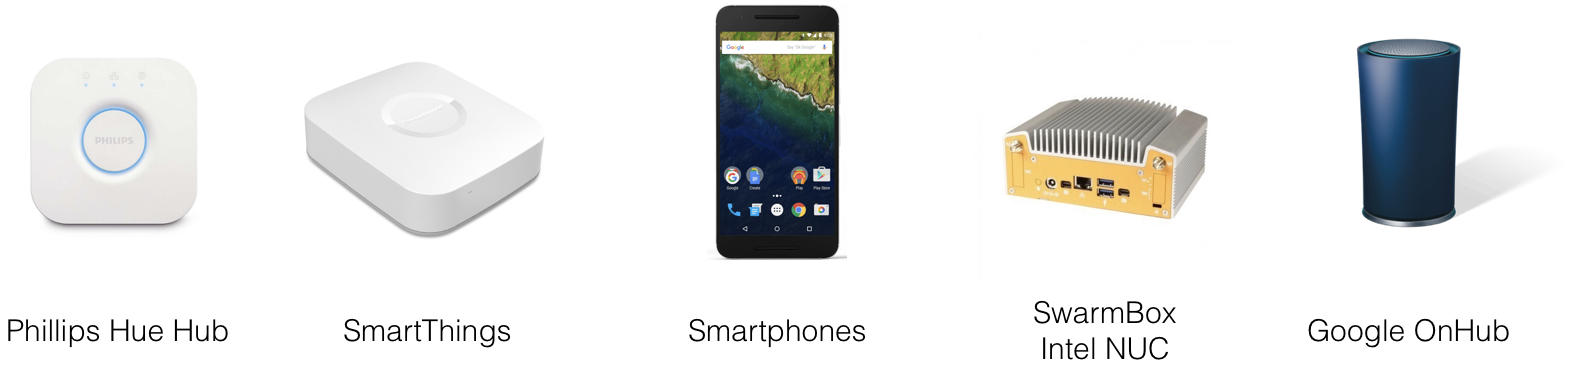
\includegraphics[width=0.8\textwidth]{figures/gateways.png}
    \captionsetup{labelformat=empty}
    \caption{Many Gateways}
  \end{figure}
\end{frame}

\begin{frame}{Heterogeneous Environment}
  \vspace{1em}
  \begin{figure}
    \centering
    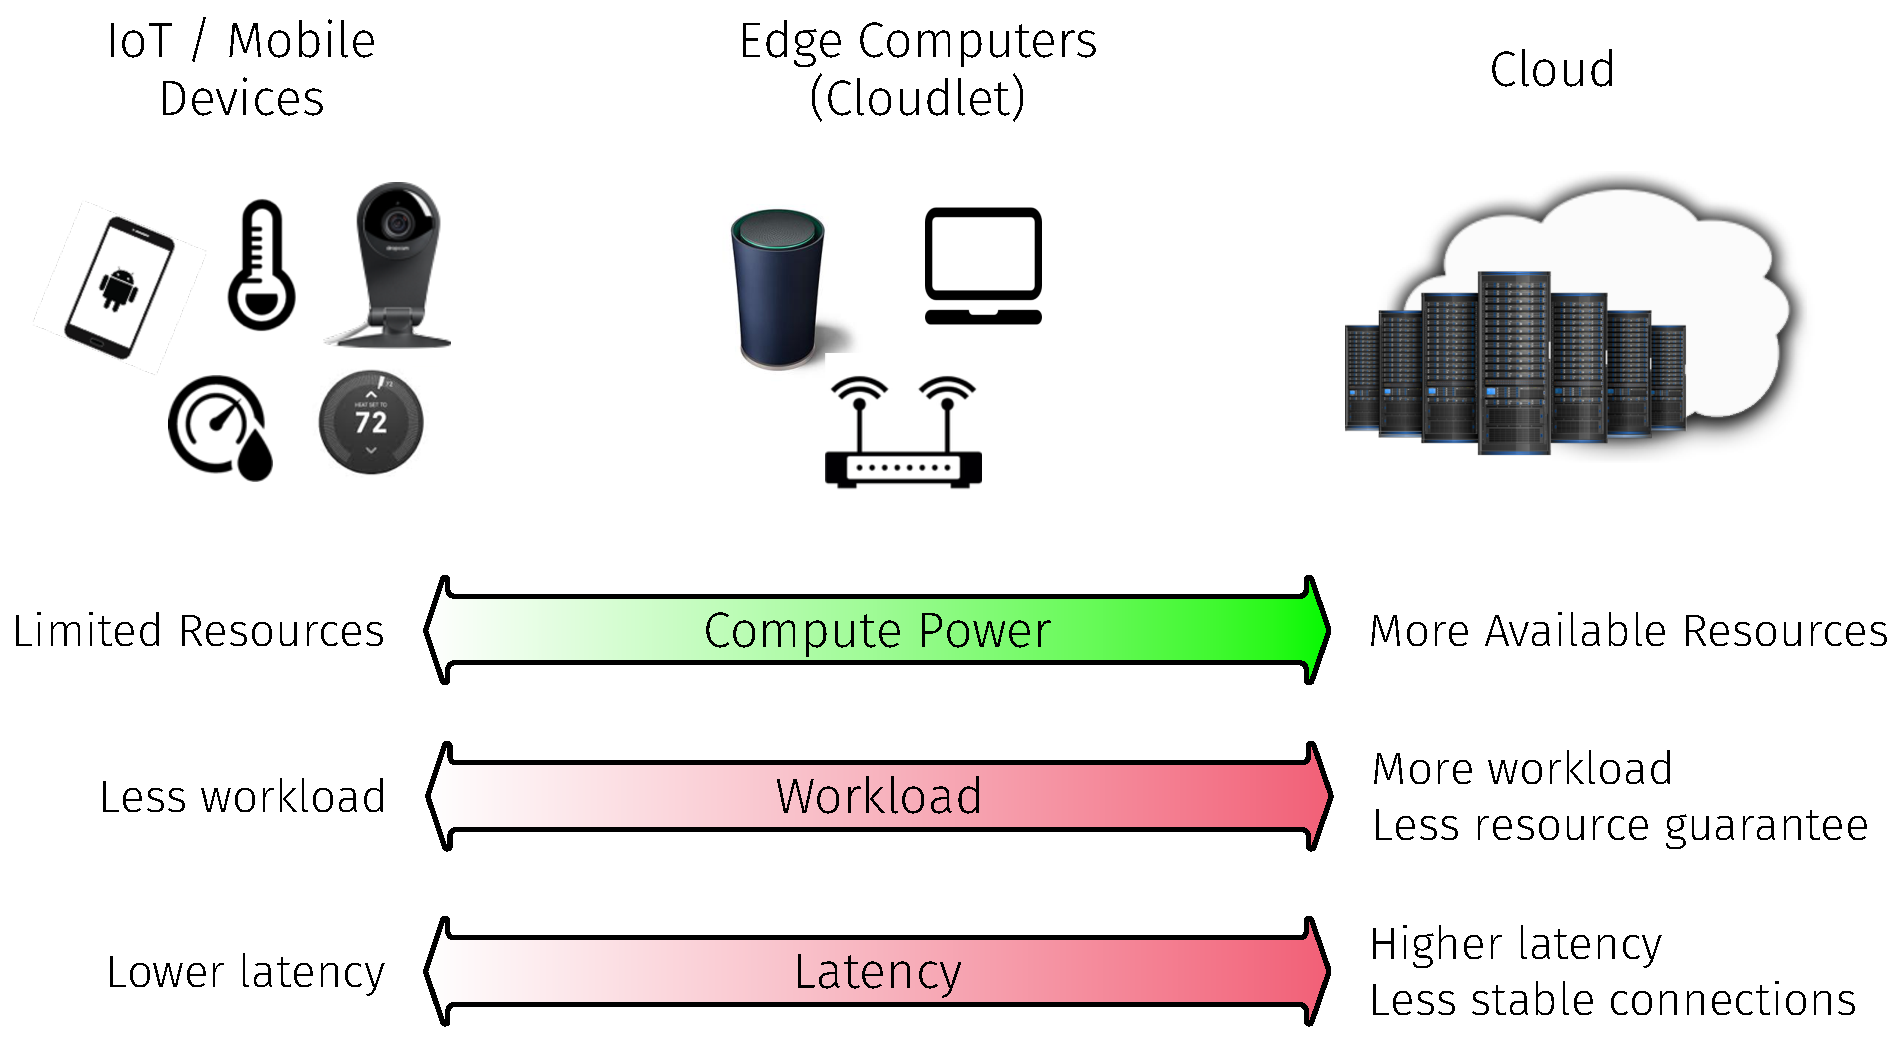
\includegraphics[width=0.95\linewidth]{figures/heterogeneous.pdf}
    \caption{Characteristics of IoT/mobile, edge and cloud}
  \end{figure}
\end{frame}

%%% Local Variables:
%%% mode: latex
%%% TeX-master: "../talk"
%%% TeX-engine: xetex
%%% End:
